\documentclass{amsart}
\usepackage{amsmath,amssymb,amsthm,fullpage,mathptmx, hyperref,dsfont,framed, graphicx, subcaption, textcomp, tikz} % The usual suspects

%%%%%%%%%%%%%%%%%% Tikz %%%%%%%%%
\usepackage{tikz}
\usetikzlibrary{shapes.geometric}
\usetikzlibrary{calc}
\usetikzlibrary{scopes}
\usetikzlibrary{decorations.markings}

\tikzset{
every picture/.style={line width=0.8pt, >=stealth,
                       baseline=-3pt,label distance=-3pt},
%%%%%%%%%%  Node styles
dotnode/.style={fill=black,circle,minimum size=2.5pt, inner sep=1pt, outer
sep=0},
morphism/.style={circle,draw,thin, inner sep=1pt, minimum size=15pt,
                 scale=0.8},
small_morphism/.style={circle,draw,thin,inner sep=1pt,
                       minimum size=10pt, scale=0.8},
coupon/.style={draw,thin, inner sep=1pt, minimum size=18pt,scale=0.8},
%%%% different line styles:
regular/.style={densely dashed},
edge/.style={thick, dashed, draw=blue, text=black},
boundary/.style={thick,  draw=blue, text=black},
overline/.style={preaction={draw,line width=2mm,white,-}},
drinfeld center/.style={>=stealth,green!60!black, double
distance=1pt,text=black},
%%%%%%% Fill styles %%%%%%%%%%%%%%%
cell/.style={fill=black!10},
subgraph/.style={fill=black!30},
%%%%%%% Mid-path arrows
midarrow/.style={postaction={decorate},
                 decoration={
                    markings,% switch on markings
                    mark=at position #1 with {\arrow{>}},
                 }},
midarrow/.default=0.5
}



\newtheorem{thm}{Theorem}[section]
\newtheorem*{uthm}{Theorem}
\newtheorem{lem}[thm]{Lemma}
\newtheorem*{ulem}{Lemma}
\newtheorem{prop}[thm]{Proposition}
%\newtheorem*{uprop}[thm]{Proposition}
\newtheorem{cor}[thm]{Corollary}
\newtheorem{conj}[thm]{Conjecture}
\newtheorem{defn}[thm]{Definition}
\newtheorem{rmk}[thm]{Remark}
\newtheorem{prob}[thm]{Open problem}
\newtheorem{ques}[thm]{Question}
\newtheorem{fact}[thm]{Fact}
\newtheorem{ex}[thm]{Exercise}


\DeclareMathOperator{\MCG}{MCG}
\DeclareMathOperator{\Vect}{Vec}
\DeclareMathOperator{\Homeo}{Homeo}
\DeclareMathOperator{\Hom}{Hom}
\DeclareMathOperator{\Obj}{Obj}
\DeclareMathOperator{\Irr}{Irr}
\DeclareMathOperator{\Img}{Im}

\begin{document}

\title{Finiteness for Mapping Class Group Representations from Twisted Dijkgraaf-Witten Theory}


\author{Paul Gustafson}
\email{pgustafs@math.tamu.edu}
\address{Department of Mathematics,
    Texas A\&M University,
    College Station, TX
    U.S.A.}
    
\maketitle
\begin{abstract}
 Every twisted Dijkgraaf-Witten representation of a mapping class group of a closed surface has finite image.
\end{abstract}

\section{Introduction}
Given a spherical category $\mathcal A$ over a field $k$ and compact surface $M$, possibly with boundary, the Turaev-Viro construction gives a projective representation of the mapping class group $\MCG(M)$.  A natural question is to determine the image of these representations.  In particular, when does such a representation have finite image?

In this setting, the Property F conjecture \cite{nr} states that, for a fixed spherical category $\mathcal A$, all associated mapping class groups are finite if and only if the Drinfeld center $Z(\mathcal A)$ is weakly integral. 

%% Do I have to talk about the center at all?  How do dimensions of objects in the center correspond the dimensions in A?

The simplest examples of spherical categories are the pointed categories, i.e. categories in which every simple object is invertible.  Every pointed category is equivalent to a category $\Vect_G^\omega$, i.e. the category of $G$-graded vector spaces with associativity given by a cocycle $\omega \in Z^3(G, k^\times)$. In this case, the Turaev-Viro construction corresponds with the twisted Dijkgraaf-Witten theory.

The center $Z(\Vect_G^\omega))$ is equivalent to the category of representations of the twisted quantum double of $G$, which is integral, so the property $F$ conjecture predicts that mapping class group representations from pointed categories should be finite. In this paper, I will verify this in the case where the surface $M$ is closed with an arbitrary finite group $G$ and cocycle $\omega$.  

\section{Related Work}

This is an extension of the result of Fjelstad and Fuchs \cite{fjfu} showing that, given a surface with at most one boundary component, the mapping class group representations corresponding to the untwisted (i.e. $\omega = 1$ case) have finite image.  However, the method of proof employed in the current paper is substantially different than theirs.  In their paper, they use an algebraic method of Lyubashenko \cite{Lyubashenko1996} that gives a projective mapping class group representation to any factorizable ribbon Hopf algebra.  In this paper, I look at the mapping class group action on a vector space of $\Vect_G^\omega$-colored embedded graphs defined by Kirillov \cite{kirillovStringNets}.

In \cite{bantay}, Bantay defined representations of mapping class groups on the Hilbert space of an orbifold model associated to $D^\omega(G)$.  These representations appear to coincide with the twisted Dijkgraaf-Witten representations. However, the connection is not clear to the current author.  Bantay even mentions that his representations are \emph{different} than TQFT representations because he treats boundary components differently.  

More is known when we fix a particular surface $M$. In the case where $M$ is a torus, it turns out that any Reshitikhin-Turaev representation of the mapping class group of the torus is always finite \cite{0806.2493}.  In particular, this implies that the Turaev-Viro representations are all finite.  In the case where $M$ is an $n$-punctured disk, the mapping class group of $M$ relative to the boundary of the disk is the braid group $B_n$.  In this case, it has been proved that the Turaev-Viro representations coming from pointed spherical categories are finite \cite{erw}.

\section{Definitions}

Let $M$ be a closed surface of genus $g$.  Let $G$ be finite group, and let $\Vect_G^\omega$ denote the category of $G$-graded vector spaces with associativity defined by the normalized 3-cocycle $\omega \in Z^3(G, k^\times)$. 

Following Kirillov \cite{kirillovStringNets}, let $H$ be the string-net vector space of $\Vect_G^\omega$-colored graph embeddings modulo null graphs. 

Let $\Gamma \in H$. Thinking of $X$ as a quotient of its fundamental polygon, by isotopy we may assume vertices of $\Gamma$ lie in the interior of the polygon and that all the edges of $\Gamma$ do not intersect corners and meet the sides transversally.  Evaluating on the interior of the polygon shows that $\Gamma$ is equivalent to a graph with a single vertex whose edges are simple closed curves, each of which intersect the boundary of the polygon precisely once.  By using the local relations, we can replace all the edges intersecting a side with a single edge labeled by the tensor product of their labels.  If there are no edges intersecting a side, we can insert a single edge labeled by the group identity into $\Gamma$ that intersects only that side.  Thus, $\Gamma$ is equivalent to a colored graph with one vertex $v$ and $2n$ outgoing edges $e_1, \ldots e_{2n}$, each of which intersects precisely one side of the fundamental polygon.


%\begin{figure}
%\begin{tikzpicture}
%\node[ellipse, scale=0.8, inner sep=1pt, draw,thin] (ph) at (3,3) 
%{$1$};

%\draw (0,0) -- (6,0)  -- (6,6) -- (0,6) -- (0,0);
%\draw (3,0) -- (ph) -- (3,6);
%\draw (0,3) -- (ph) -- (6,3);

%\end{tikzpicture}
%\caption{Element of the spanning set for the torus}
%\end{figure}


By the definition of the evaluation of a string-net and the definition of the quotient map identifying the sides of the fundamental polygon, the vertex $v$ is colored by an element $\phi(v) \in \Hom_{\Vect_G^\omega} (1, \bigotimes_{i=1}^n V(e_{2i-1}) \otimes V(e_{2i})  \otimes V(e_{2i-1}^*) \otimes V(e_{2i}^*))$, where $V(e_i) \in \Obj(\Vect_G^\omega)$ is the coloring of the edge $e_i$.  Since string-net evaluation is additive in the direct sum and linear in the vertex color, it follows that $H$ is spanned by the set of colored graphs
$$ S := \{\Gamma \in H : V(e_i) \in \Irr(\Vect_G^\omega), \phi(v) = 1 \}, $$
where $\Irr(\Vect_G^\omega)$ is the set of simple objects of $\Vect_G^\omega$.  See Figure \ref{fig:span} for a depiction.

\begin{figure}
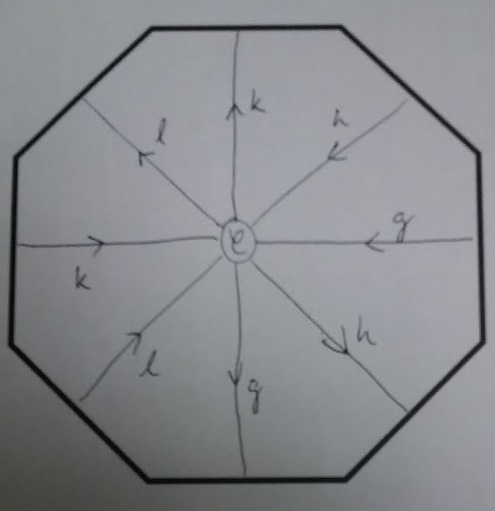
\includegraphics[width=0.5\textwidth]{basis.jpg}
\caption{Element of the spanning set $S$ for a genus 2 surface}
\label{fig:span}
\end{figure}


%% The action of the mapping class group on H

\begin{prop}
The action of the mapping class group on the vector space $H$ induced by the action of the orientation-preserving homeomorphisms on the surface $M$ is well-defined.
\end{prop}
\begin{proof}
The orientation-preserving group $\Homeo^+(M)$ acts on colored embedded graphs in $M$.  To see that the mapping class group $\MCG(M)$ has a well-defined action on $H$, we need to check two things: first, that isotopic homeomorphisms acting on a colored graph take it to equivalent colored graphs and, second, that a homeomorphism maps equivalent colored graphs to equivalent colored graphs.

For the first, suppose $f, g \in Homeo^+(M)$ are isotopic, with $H: M \times I \to M$ an isotopy from $f$ to $g$.  Let $i: \Gamma \to M$ be an graph embedding.  Then $H \circ i$ is an isotopy from $f \circ i$ to $g \circ i$.    

For the second,  to check that a homeomorphism $f \in \Homeo^+(M)$ preserves equivalence of colored graphs, it suffices to check that it in the case of each local move.  Since the mapping class group is generated by Dehn twists, all the local moves reduce to the isotopy move. 

To check that isotopic colored graphs get mapped to equivalent colored graphs, suppose $\Gamma$ is a graph and $i: \Gamma to M$ and $j: \Gamma \to M$ are isotopic embeddings. Let $H: \Gamma \times I \to M$ be an isotopy from $i$ to $j$.  Let $f \in \Homeo^+(M)$.  Then $f \circ H$ is an isotopy from $f \circ i$ to $f \circ j$.  

Thus, the action of the mapping class group on $H$ is well-defined.
\end{proof}

%% The action of H on the spanning set

\begin{thm}
The image of the twisted Dijkgraaf-Witten representation of a mapping class group of any closed surface $M$ is finite.
\end{thm}

\begin{proof}
The mapping class group of $M$ is generated by the Lickorish generating set consisting of Dehn twists around $3g-1$ simple closed curves (see Figure \ref{fig:lickorish}).  These can be divided into two types of twists: the ones around a single hole, and the ones connecting two holes.

\begin{figure}
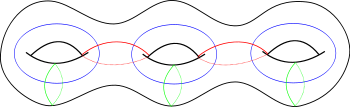
\includegraphics[width=.80\textwidth]{lickorish.png}
\caption{Lickorish generating set}
\label{fig:lickorish}
\end{figure}

\newcommand{\nc}{\newcommand}

%% Definitions

    % boundary of polygon
    % top left corner
     \nc{\lcx}{-0.5}
     \nc{\lcy}{0.866}
     \nc{\rcx}{-\lcx}
     \nc{\rcy}{\lcy}

     %TODO: Color edges
     \nc{\makeBdy}{
       \begin{scope}[very thick,decoration={
             markings,
             mark=at position 0.5 with {\arrow{>}}}
         ]  

         \draw[postaction={decorate}] (-1,0) -- (\lcx, \lcy); 
         \draw (\lcx, \lcy) -- (\rcx, \rcy); 
         \draw[postaction={decorate}]  (1, 0) -- (\rcx, \rcy);
       \end{scope}
     }

    %cut    
    % left endpoint of cut
    \nc{\lcutx}{-0.6}
    \nc{\lcuty}{0.6928}
    \nc{\lcut}{(\lcutx, \lcuty)}
    \nc{\rcutx}{-\lcutx}
    \nc{\rcuty}{\lcuty}
    \nc{\rcut}{(\rcutx, \rcuty)}

    %Main vertex
    \nc{\mvx}{0}
    \nc{\mvy}{0.2}
    \nc{\mv}{(\mvx, \mvy)}

    % outgoing edge
    \nc{\outEdge}{\draw[postaction={decorate}]  (0, 0) -- \mv node[pos=.5, right]{$hgh^{-1}$};}

    % middle of top edge of polygon
    \nc{\mtopx}{0}
    \nc{\mtopy}{0.866}
    \nc{\mtop}{(\mtopx, \mtopy)}


%Dehn twist 1.1
\begin{figure}
    \centering
    \begin{tikzpicture}[scale=5]    

      
      % boundary of polygon
      \makeBdy


    \begin{scope}[very thick,decoration={
    markings,
    mark=at position 0.5 with {\arrow{>}}}
    ]  

      % cut for Dehn twist
      \draw[loosely dashed] \lcut -- \rcut;
      

      %graph edges

      \draw[postaction={decorate}]   \mv -- (0.75, 0.433) node[pos=.5,sloped,above]{$h$};
      \draw[postaction={decorate}]   \mv -- \mtop node[pos=.5,left]{$g$};
      \draw[postaction={decorate}]  (-0.75, 0.433) -- \mv node[pos=.5,sloped,above]{$h$};
      \outEdge

    \end{scope}
    \end{tikzpicture}
    \caption{First type of Dehn twist}
    \label{fig:tikzTwist1_1}
\end{figure}



%1.2
\begin{figure}
    \centering
    \begin{tikzpicture}[scale=5]
    
    %boundary of polygon
      \makeBdy

    %graph edges
    \begin{scope}[very thick,decoration={
    markings,
    mark=at position 0.5 with {\arrow{>}}}
    ] 


        \draw[postaction={decorate}]   \mv -- (0.75, 0.433) node[pos=.5,sloped,above]{$h$};
        % old g
        % \draw[postaction={decorate}]   \rb -- (0, 0.866) node[pos=.5,left]{$g$};
        \draw[postaction={decorate}]  (-0.75, 0.433) -- \mv node[pos=.5,sloped,above]{$h$};
        \outEdge

        % new g
        \draw[postaction={decorate}]  \mv -- \rcut
        node[pos=.5,sloped,above]{$g$};
        \draw[postaction={decorate}]  \lcut -- \mtop
        node[pos=.5,sloped,below]{$g$};

    \end{scope}
    \end{tikzpicture}
    \caption{First type of Dehn twist}
    \label{fig:tikzTwist1_2}
\end{figure}


%1.3
\begin{figure}
    \centering
    \begin{tikzpicture}[scale=5]
    
    %boundary of polygon
      \makeBdy

    %graph edges
    \begin{scope}[very thick,decoration={
    markings,
    mark=at position 0.5 with {\arrow{>}}}
    ] 

        \draw[postaction={decorate}]   \mv -- (0.75, 0.433) node[pos=.5,sloped,above]{$h$};
        \draw[postaction={decorate}]  (-0.75, 0.433) -- \mv node[pos=.5,sloped,above]{$h$};

        \outEdge

        \draw[postaction={decorate}]  \mv -- \rcut
        node[pos=.5,sloped,above]{$g$};
        %\draw[postaction={decorate}]  \lcut -- \mtop
        \draw[postaction={decorate}]  \lcut --  ({(\lcutx + \mtopx)/2} , {(\lcuty + \mtopy)/2})
        node[pos=.5,sloped,below]{$g$};
        \draw[postaction={decorate}]  ({(\lcutx + \mtopx)/2} , {(\lcuty + \mtopy)/2}) -- \mtop
        node[pos=.5,sloped,below]{$g$};


        \draw  \mv --  ({(\lcutx + \mtopx)/2} , {(\lcuty + \mtopy)/2});

    \end{scope}
    \end{tikzpicture}
    \caption{First type of Dehn twist}
    \label{fig:tikzTwist1_3}
\end{figure}


%1.4
\begin{figure}
    \centering
    \begin{tikzpicture}[scale=5]

      %boundary of polygon
      \makeBdy


      
      \begin{scope}[very thick,decoration={
            markings,
            mark=at position 0.5 with {\arrow{>}}}
        ] 
      %graph edges

        \draw[postaction={decorate}]   \mv -- (0.75, 0.433) node[pos=.5,sloped,above]{$h$};
        \draw[postaction={decorate}]  (-0.75, 0.433) -- \mv node[pos=.5,sloped,above]{$h$};

        \outEdge

        \draw[postaction={decorate}]  \mv -- \rcut
        node[pos=.5,sloped,above]{$g$};
        %\draw[postaction={decorate}]  \lcut -- \mtop
        \draw[postaction={decorate}]  \lcut -- \mv
        node[pos=.5,sloped,above]{$g$};
        \draw[postaction={decorate}]  \mv -- \mtop
        node[pos=.5,right]{$g$};


    \end{scope}
    \end{tikzpicture}
    \caption{First type of Dehn twist}
    \label{fig:tikzTwist1_4}
\end{figure}



%Dehn twist 1.5
\begin{figure}
    \centering
    \begin{tikzpicture}[scale=5]

    % boundary of polygon
     \makeBdy
    
    %graph edges
    \begin{scope}[very thick,decoration={
    markings,
    mark=at position 0.5 with {\arrow{>}}}
    ]  
        \draw[postaction={decorate}]   \mv -- (0.75, 0.433) node[pos=.5,sloped,above]{$hg$};
        \draw[postaction={decorate}]   \mv -- \mtop node[pos=.5,left]{$g$};
        \draw[postaction={decorate}]  (-0.75, 0.433) -- \mv node[pos=.5,sloped,above]{$hg$};
        \outEdge

    \end{scope}
    \end{tikzpicture}
    \caption{First type of Dehn twist}
    \label{fig:tikzTwist1_5}
\end{figure}

%%%%%%%%%%%% Twist 2 %%%%%%%%%%%%%%%%


\nc{\makeBdyTwo}{
  \begin{scope}[very thick,decoration={
    markings,
    mark=at position 0.5 with {\arrow{>}}}
    ]  
    \path[draw]
    (1.0,          0.0) --       %0
    (0.92388,      0.382683)  -- %1
    (0.707107,     0.707107) --  %2
    (0.382683,     0.92388) --   %3
    (0,            1.0)   --     %4
    (-0.382683,    0.92388) --   %5
    (-0.707107 ,   0.707107)  -- %6
    ( -0.92388,    0.382683) --  %7
    ( -1.0     ,   0);           %8

  \end{scope}
}

\nc{\outEdgeTwo}{\draw[postaction={decorate}]  (0, 0) -- \mv node[pos=.5, right]{$[a,b][c,d]$};}

% 0.9 1 + 0.1 6
\nc{\cutOneX}{{0.8*(-0.92388) + 0.2*(-0.707107)}}
\nc{\cutOneY}{{0.8*(0.382683) + 0.2*(0.707107)}}
\nc{\cutOne}{(\cutOneX, \cutOneY)}

%0.9 3 + 0.1 4
\nc{\cutTwoX}{{0.8*(0.382683) + 0.2*(0)}}
\nc{\cutTwoY}{{0.8*(0.92388) + 0.2*(1.0)}}
\nc{\cutTwo}{(\cutTwoX, \cutTwoY)}

%0.9 2 + 0.1 1
\nc{\cutThreeX}{{0.8*(0.707107 ) + 0.2*(0.92388 )}}
\nc{\cutThreeY}{{0.8*(0.707107 ) + 0.2*(0.382638 )}}
\nc{\cutThree}{(\cutThreeX, \cutThreeY)}

%0.9 2 + 0.1 3
\nc{\cutFourX}{{0.2*( 0.382683) + 0.8*(0.707107)}}
\nc{\cutFourY}{{0.2*( 0.92388) + 0.8*(0.707107)}}
\nc{\cutFour}{(\cutFourX, \cutFourY)}

%0.1 0   0.9 1
\nc{\cutFiveX}{{0.2*( 1.0) + 0.8*(0.92388)}}
\nc{\cutFiveY}{{0.2*( 0.0) + 0.8*(0.382638)}}
\nc{\cutFive}{(\cutFiveX, \cutFiveY)}

%0.1 2   0.9 1
\nc{\cutSixX}{{0.2*( 0.707107) + 0.8*(0.92388)}}
\nc{\cutSixY}{{0.2*( 0.707107) + 0.8*(0.382683)}}
\nc{\cutSix}{(\cutSixX, \cutSixY)}

%0.1 3      0.9 4
\nc{\cutSevenX}{{0.2*( 0.382683) + 0.8*(0.0)}}
\nc{\cutSevenY}{{0.2*( 0.92388) + 0.8*(1.0)}}
\nc{\cutSeven}{(\cutSevenX, \cutSevenY)}

%0.1 5 0.9 4
\nc{\cutEightX}{{0.2*( -0.382683) + 0.8*(0.0)}}
\nc{\cutEightY}{{0.2*( 0.92388) + 0.8*(1.0)}}
\nc{\cutEight}{(\cutEightX, \cutEightY)}

\begin{figure}
    \centering
    \begin{tikzpicture}[scale=8]

    % boundary of polygon
     \makeBdyTwo

     % cut for Dehn twist
     \draw[dotted] \cutOne -- \cutTwo;
     \draw[dotted] \cutThree -- \cutFour;
     \draw[dotted] \cutFive -- \cutSix;
     \draw[dotted] \cutSeven -- \cutEight;
         
    %graph edges
    \begin{scope}[very thick,decoration={
    markings,
    mark=at position 0.5 with {\arrow{>}}}
    ]  
       \draw[postaction={decorate}]  \mv -- (   0.96194 , 0.191342) node[pos=.5,sloped,above]{$a$};
       \draw[postaction={decorate}]  \mv -- ( 0.815493,  0.544895) node[pos=.5,sloped,above]{$b$};
       \draw[postaction={decorate}] (0.544895,  0.815493) -- \mv  node[pos=.5,sloped,above]{$a$};
       \draw[postaction={decorate}]   (0.191342,  0.96194) -- \mv  node[pos=.5,sloped,above]{$b$}; 
       \draw[postaction={decorate}]  \mv -- (-0.191342,  0.96194) node[pos=.5,sloped,above]{$c$}; 
       \draw[postaction={decorate}]  \mv -- (-0.544895,  0.815493) node[pos=.5,sloped,above]{$d$}; 
       \draw[postaction={decorate}] (-0.815493,  0.544895) -- \mv  node[pos=.5,sloped,above]{$c$};
       \draw[postaction={decorate}] (-0.96194,   0.191342) -- \mv  node[pos=.5,sloped,above]{$d$};

         \outEdgeTwo
    \end{scope}
    \end{tikzpicture}
    \caption{Second type of Dehn twist}
    \label{fig:tikzTwist2_1}
\end{figure}




 Using the local moves as in Figures \ref{fig:dehn1} and \ref{fig:dehn2}, one sees that the result of each of these Dehn twists lies in $\Img(\omega) S$.  It is a basic result in group cohomology that, by replacing $\omega$ with a cohomologous cocycle if necessary, $\Img(\omega) \subset \mu_{|G|}$, where $\mu_{|G|} \subset k^\times$ is the finite set of $|G|$-th roots of unity.  

Thus, the image of any such mapping class group representation is finite.
\end{proof}

\medskip
 
\bibliographystyle{unsrt}
\bibliography{stringnets}







\end{document}
